
\chapter{Building graphs with bundled vertices}
\label{sec:Building-graphs-with-bundled-vertices}
%%%%%%%%%%%%%%%%%%%%%%%%%%%%%%%%%%%%%%%%%%%%%%%%%%%%%%%%%%%%%%%%%%%%%%%%%%%%%%%%

Up until now, the graphs created have had edges and vertices without any
properties.
In this chapter, graphs will be created, in which the vertices can have
a bundled \verb;my_bundled_vertex; type
\footnote{I do not intend to be original in naming my data types}.
The following graphs will be created:

\begin{itemize}
  \item An empty directed graph that allows for bundled vertices: 
    see chapter \ref{lst:create_empty_directed_bundled_vertices_graph}
  \item An empty undirected graph that allows for bundled vertices: 
    see chapter \ref{subsec:create_empty_directed_bundled_vertices_graph}
  \item A two-state Markov chain with bundled vertices: 
    see chapter \ref{subsec:create_bundled_vertices_markov_chain}
  \item $K_{2}$ with bundled vertices: 
    see chapter \ref{subsec:create_bundled_vertices_k2_graph}
\end{itemize}

In the process, some basic (sometimes bordering trivial) functions are shown:

\begin{itemize}
  \item 
    Create the vertex class, called \verb;my_bundled_vertex;: 
    see chapter \ref{subsec:my_bundled_vertex}
  \item Adding a \verb;my_bundled_vertex;: 
    see chapter \ref{subsec:add_bundled_vertex}
  \item Getting the vertices \verb;my_bundled_vertex;-es: 
    see chapter \ref{subsec:get_bundled_vertex_my_vertexes}
\end{itemize}

These functions are mostly there for completion and showing which data types
are used.

%%%%%%%%%%%%%%%%%%%%%%%%%%%%%%%%%%%%%%%%%%%%%%%%%%%%%%%%%%%%%%%%%%%%%%%%%%%%%%%%
\section{Creating the bundled vertex class}
\label{subsec:my_bundled_vertex}
%%%%%%%%%%%%%%%%%%%%%%%%%%%%%%%%%%%%%%%%%%%%%%%%%%%%%%%%%%%%%%%%%%%%%%%%%%%%%%%%

Before creating an empty graph with bundled vertices, that bundled vertex
class must be created.
In this tutorial, it is called \verb;my_bundled_vertex;.
\verb;my_bundled_vertex; is a class that is nonsensical, but it can be replaced
by any other class type.

Here I will show the header file of \verb;my_bundled_vertex;, as the implementation
of it is not important:

\lstinputlisting[
  caption = Declaration of my\_bundled\_vertex,
  label = lst:my_bundled_vertex_h
]{my_bundled_vertex.impl}
\index{my_bundled_vertex}
\index{my_bundled_vertex.h}
\index{my_vertex declaration}
\index{Declaration, my_bundled_vertex}

\verb;my_bundled_vertex; is a class that has multiple properties: 

\begin{itemize}
  \item
    It has four public member variables: 
    the double \verb;m_x; 
    (\verb;m_; \index{m\_} stands for 'member' \index{member}), 
    the double \verb;m_y;, 
    the \verb;std::string; \verb;m_name; and the 
    \verb;std::string; \verb;m_description;.
    These variables must be public
  \item It has a default constructor
  \item It is copyable
  \item It is comparable for equality 
    (it has \verb;operator==;), 
    which is needed for searching
\end{itemize}

\verb;my_bundled_vertex; does not have to have the stream operators defined for
file I/O, as this goes via the public member variables.

%%%%%%%%%%%%%%%%%%%%%%%%%%%%%%%%%%%%%%%%%%%%%%%%%%%%%%%%%%%%%%%%%%%%%%%%%%%%%%%%
\section{Create the empty directed graph with bundled vertices}
\label{subsec:create_empty_directed_bundled_vertices_graph}
%%%%%%%%%%%%%%%%%%%%%%%%%%%%%%%%%%%%%%%%%%%%%%%%%%%%%%%%%%%%%%%%%%%%%%%%%%%%%%%%

\lstinputlisting[
  caption = Creating an empty directed graph with bundled vertices,
  label = lst:create_empty_directed_bundled_vertices_graph
]{create_empty_directed_bundled_vertices_graph.impl}
\index{Create empty directed bundled vertices graph}

This graph:

\begin{itemize}
  \item has its out edges stored in a std::vector 
    (due to the first boost::vecS \index{boost::vecS})
  \item has its vertices stored in a std::vector 
    (due to the second boost::vecS \index{boost::vecS})
  \item is directed 
    (due to the boost::directedS \index{boost::directedS})
  \item The vertices have one property: 
    they have a bundled type, 
    that is of data type \verb;my_bundled_vertex;
  \item The edges and graph have no properties
  \item Edges are stored in a std::list
\end{itemize}

The \verb;boost::adjacency_list; has a new, fourth template argument 
\verb;my_bundled_vertex; \index{my_bundled_vertex}.

This can be read as: 

\begin{quote}
vertices have the bundled property \verb;my_bundled_vertex;
\end{quote}

Or simply: 

\begin{quote}
vertices have a bundled type called \verb;my_bundled_vertex;
\end{quote}

%%%%%%%%%%%%%%%%%%%%%%%%%%%%%%%%%%%%%%%%%%%%%%%%%%%%%%%%%%%%%%%%%%%%%%%%%%%%%%%%
\section{Create the empty undirected graph with bundled vertices}
\label{subsec:create_empty_undirected_bundled_vertices_graph}
%%%%%%%%%%%%%%%%%%%%%%%%%%%%%%%%%%%%%%%%%%%%%%%%%%%%%%%%%%%%%%%%%%%%%%%%%%%%%%%%

\lstinputlisting[
  caption = Creating an empty undirected graph with bundled vertices,
  label = lst:create_empty_undirected_bundled_vertices_graph
]{create_empty_undirected_bundled_vertices_graph.impl}
\index{Create empty undirected bundled vertices graph}

This code is very similar to the code described 
in chapter \ref{subsec:create_empty_directed_bundled_vertices_graph}, 
except that the directness (the third template argument) is undirected 
(due to the boost::undirectedS \index{boost::undirectedS}).

%%%%%%%%%%%%%%%%%%%%%%%%%%%%%%%%%%%%%%%%%%%%%%%%%%%%%%%%%%%%%%%%%%%%%%%%%%%%%%%%
\section{Add a bundled vertex}
\label{subsec:add_bundled_vertex}
%%%%%%%%%%%%%%%%%%%%%%%%%%%%%%%%%%%%%%%%%%%%%%%%%%%%%%%%%%%%%%%%%%%%%%%%%%%%%%%%

Adding a bundled vertex is very similar to adding a named vertex 
(chapter \ref{subsec:add_named_vertex}).

\lstinputlisting[
  caption = Add a bundled vertex,
  label = lst:add_bundled_vertex
]{add_bundled_vertex.impl}
\index{Add bundled vertex}

When having added a new (abstract) vertex to the graph, the vertex descriptor
is used to set the \verb;my_bundled_vertex; in the graph.

%%%%%%%%%%%%%%%%%%%%%%%%%%%%%%%%%%%%%%%%%%%%%%%%%%%%%%%%%%%%%%%%%%%%%%%%%%%%%%%%
\section{Getting the bundled vertices' my\_vertexes}
\footnote{
  the name my\_vertexes; is chosen to allows you to
  replace my\_vertex by your favorite datatype name,
  although in English the plural of vertex is vertices
}
\label{subsec:get_bundled_vertex_my_vertexes}
%%%%%%%%%%%%%%%%%%%%%%%%%%%%%%%%%%%%%%%%%%%%%%%%%%%%%%%%%%%%%%%%%%%%%%%%%%%%%%%%

When the vertices of a graph have any bundled \verb;my_bundled_vertex;, one can
extract these as such:

\lstinputlisting[
  caption = Get the bundled vertices' my\_vertexes,
  label = lst:get_my_bundled_vertexes
]{get_my_bundled_vertexes.impl}
\index{Get bundled vertex my_vertexes}

The \verb;my_bundled_vertex; bundled in each vertex is obtained from a vertex
descriptor and then put into a std::vector.

The order of the \verb;my_bundled_vertex; objects may be different after saving
and loading.
When trying to get the vertices' my_bundled_vertex from a graph without
 these, you will get the error 
\verb;formed reference to void; (see chapter \ref{subsec:formed_reference_to_void}).

%%%%%%%%%%%%%%%%%%%%%%%%%%%%%%%%%%%%%%%%%%%%%%%%%%%%%%%%%%%%%%%%%%%%%%%%%%%%%%%%
\section{Creating a two-state Markov chain with bundled vertices}
\label{subsec:create_bundled_vertices_markov_chain}
%%%%%%%%%%%%%%%%%%%%%%%%%%%%%%%%%%%%%%%%%%%%%%%%%%%%%%%%%%%%%%%%%%%%%%%%%%%%%%%%

\subsection{Graph}

Figure \ref{fig:bundled_vertices_markov_chain} 
shows the graph that will be reproduced:

\begin{figure}
  \begin{tikzpicture}
    \draw[->,>=stealth',shorten >=1pt,auto,node distance=4cm, semithick]
    \tikzstyle{every state}=[]
    \node[state] (A) 
        {Sunny, Yellow, 1.0, 2.0};   
    \node[state] (B) [right of=A] 
        {Not rainy, Not grey, 3.0, 4.0}
      ;   
    \path (A) edge [loop  left] node {} (A)
          (A) edge [bend  left] node {} (B)
          (B) edge [bend  left] node {} (A)
          (B) edge [loop right] node {} (B); 
  \end{tikzpicture}
  \caption{
    A two-state Markov chain where the vertices have bundled properties and
    the edges have no properties.
    The vertices' properties are nonsensical
  }
  \label{fig:bundled_vertices_markov_chain}
\end{figure}

\subsection{Function to create such a graph}

Here is the code creating a two-state Markov chain with bundled vertices:

\lstinputlisting[
  caption = Creating the two-state Markov chain as depicted in figure \ref{fig:bundled_vertices_markov_chain},
  label = lst:create_bundled_vertices_markov_chain
]{create_bundled_vertices_markov_chain.impl}
\index{Create bundled vertices Markov chain}

\subsection{Creating such a graph}

Here is the demo:

\lstinputlisting[
  caption = Demo of the create\_bundled\_vertices\_markov\_chain function (algorithm \ref{lst:create_bundled_vertices_markov_chain}),
  label = lst:create_bundled_and_vertices_markov_chain_demo
]{create_bundled_vertices_markov_chain_demo.impl}

\subsection{The .dot file produced}

\lstinputlisting[
  caption = .dot file created from the create\_bundled\_vertices\_markov\_chain function (algorithm \ref{lst:create_bundled_vertices_markov_chain}) converted from graph to .dot file using algorithm \ref{lst:save_bundled_vertices_graph_to_dot},
  label = lst:create_bundled_vertices_markov_chain.dot
]{create_bundled_vertices_markov_chain.dot}

\subsection{The .svg file produced}

\begin{figure}[!htbp]
  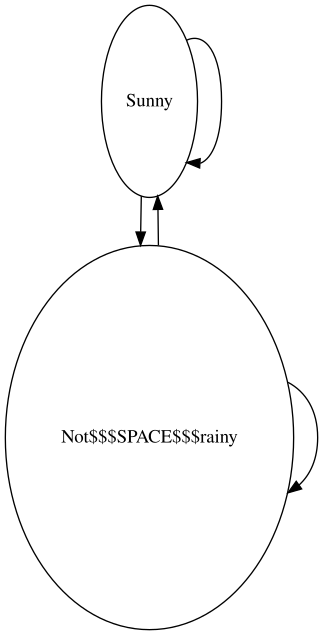
\includegraphics[]{create_bundled_vertices_markov_chain.svg}
  \caption{
    .svg file created from the create\_bundled\_vertices\_markov\_chain function
    (algorithm \ref{lst:create_bundled_vertices_markov_chain}) 
    its .dot file, converted from .dot file to .svg 
    using algorithm \ref{lst:convert_dot_to_svg}
  }
  \label{fig:create_bundled_vertices_markov_chain.svg}
\end{figure}

